\documentclass[10pt,a4paper]{article}
\usepackage[utf8]{inputenc}
\usepackage[german]{babel}
\usepackage{amsmath}
\usepackage{amsfonts}
\usepackage{amssymb}
\usepackage{siunitx}
\usepackage[left=2cm,right=2cm,top=2cm,bottom=2cm]{geometry}
\usepackage{wrapfig}
\usepackage{graphicx}
\usepackage[outdir=./figures/]{epstopdf}
\usepackage{capt-of}
\usepackage{multirow}
\usepackage[colorlinks]{hyperref}
\usepackage[section]{placeins}
\usepackage{booktabs}

\author{Christian Bespin \and Christopher Deutsch}
\title{Übungsblatt 5: Numerische Methoden der Physik}
\begin{document}
\maketitle

\setcounter{section}{4}

\section{Wärmeleitung}

\subsection{Physikalischer Hintergrund}
Grundlage für Wärmeaustauschvorgänge, wie die hier zu behandelnde Wärmeleitung, bildet das \emph{Fourier'sche Gesetz}. Es besagt, dass die Wärmestromdichte $\dot{\vec{q}}$ durch ein Flächenstück proportional zum negativen Temperaturgradienten auf der Oberfläche ist. Aus der Energieerhaltung folgt, dass diese Änderung der Energie gleich der aus Quellen zugeflossenen und über die Fläche abfließenden Energie ist. Wir erhalten dann für die Temperatur $u(x)$ am Ort $x$ auf dem Flächenstück:
\begin{align}  
\frac{\partial}{\partial t}u(\vec{x},t)=f(\vec{x},t)+ a \Delta u(\vec{x},t)
\end{align}
Dabei beschreibt $f(x)$ die Wärmequellen und -senken und $a$ die Temperaturleitfähigkeit, die bei der Bearbeitung der Aufgabe gleich $1$ gesetzt wird. Da wir bei der Aufgabe den stationären Fall betrachten, ist die zeitliche Ableitung konstant und $u$ und $f$ reduzieren sich auf Funktionen, die nur vom Ort $x$ abhängen.

\subsection{Numerische Methoden}
\subsubsection{Diskretisierung des Laplace-Operators}
Zur Bearbeitung der Aufgabe muss das betrachtete, zusammenhängende Gebiet in diskrete Teilstücke zerlegt werden, um das Problem numerisch zu lösen, dabei müssen die verwendeten Operatoren ebenfalls diskretisiert werden. Hierfür wird ein isotropes Gitter mit festem Gitterabstand $a$ in alle Richtungen gewählt. Mit Hilfe des Einheitsvektors in $\mu$-Richtung können von jedem Punkt $\vec{x}$ ausgehend mit $\vec{x} \pm a\vec{\mu}$ die Nachbarpunkte eines Gitterpunktes erreichen.

Zur Diskretisierung des Laplace-Operators ist es notwendig, die zweiten Ableitung nach der Ortskoordinate zu berechnen. Dies geschieht mit Hilfe des zentralen Differenzenquotient:
\begin{align}
\frac{\partial u(\vec{x})}{\partial x_{\mu}}=\frac{u(\vec{x}+\frac{a}{2}\vec{\mu}) - u(x-\frac{a}{2}\vec{\mu})}{a}
\label{eqn:diffquotient1}
\end{align}

Die zweite Ableitung kann nun durch die zweifache Anwendung von (\ref{eqn:diffquotient1}) an den Gitterpunkten genähert werden:
\begin{align}
\frac{\partial^2 u(\vec{x})}{\partial x_{\mu}^2}=\frac{u(\vec{x}+a\vec{\mu})-2 u(\vec{x})+u(x-a\vec{\mu})}{a^2}
\label{eqn:diffquotient2}
\end{align}

Verschieben: Dieses Verfahren ist besonders für die Neumann Randbedingung wie in  \ref{randbedingungen} interessant, denn man erkennt, dass man das betrachtete Gebiet in diesem speziellen Fall über den Rand fortsetzen kann. Dies geschieht gerade mit $f_{x+a\vec{\mu}}=f_{x-a\vec{\mu}}$, denn dann verschwindet die erste Ableitung (als Differenzenquotient wie in \ref{eqn:diffquotient2} ausgedrückt), wie die Randbedingung fordert.

Man erhält durch die Diskretisierung also ein Gleichungssystem mit einer dünn besetzten Matrix, deren Einträge die Gitterpunkte repräsentieren. Die Lösung solcher Systeme (insbesondere für dünn besetzte Matrizen) wird im nachfolgenden Abschnitt \ref{sec:gauss-seidel} erläutert.

\begin{figure}[htbp!]
\centering
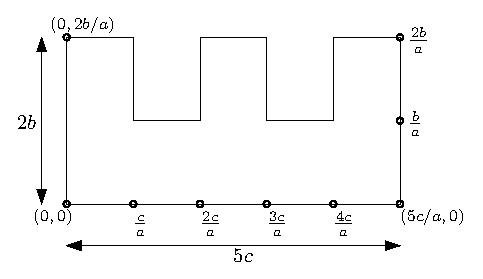
\includegraphics[height=5cm]{./figures/grid.eps}
\end{figure}

\subsubsection{Differentialgleichung}

\subsubsection{Randbedingungen}
\label{randbedingungen}
Bei der zu bearbeitenden Aufgabe tauchen zwei verschiedene Randbedingungen auf:
\begin{itemize}
\item Dirichlet Randbedingungen und
\item Neumann Randbedingungen
\end{itemize}
Die Dirichlet-Randbedingung geben einen festen Wert für die Funktion $u$ in (FEHLENDE REFERENZ) auf dem Rand des betrachteten Gebietes vor. In unserem Fall werden sowohl für $f$ als auch $u$ konstante Werte auf dem Rand des Objektes angegeben. Die Neumann Randbedingung legt einen Wert für $\frac{\partial u}{\partial \vec{\mu}}$ auf dem Rand fest, wobei $\vec{\mu}$ der nach außen gerichtete Normalenvektor auf dem Rand ist. Die Aufgabe gibt für $\frac{\partial u}{\partial \vec{\mu}}$ den Wert $0$ auf der unteren Kante vor. Sie besagt, dass von dem Rand keine Wärmeleitung nach außen stattfindet, und die Wärme von der Kante über das Objekt abfließt.

\subsubsection{Gauß-Seidel Verfahren}
\label{sec:gauss-seidel}
Zur Lösung des Gleichungssystems nutzen wir das für große, dünne Matrizen gut geeignete Iterationsverfahren nach \emph{Gauß-Seidel}. Dazu wird das Gleichungssystem $A\vec{x}=\vec{b}$ in Fixpunktform geschrieben:
\begin{align}
\vec{x}^{\,k+1}=H\vec{x}^{\,k}+\vec{c}
\end{align}
Hierbei ist $H=1-B^{-1}A$ und $\vec{c}=B^{-1}\vec{b}$, wobei $B$ so gewählt wird, dass $B^{-1}\approx A^{-1}$. Weiterhin soll $B$ leicht zu invertieren sein. Nimmt man an, dass die Diagonalelemente von A $\not=0$ sind, kann man das Gleichungssystem zeilenweise lösen. Dazu betrachtet man die $i$-te Zeile
\begin{align}
a_{i0}\,x_0+...+a_{i,n-1}\,x_{n-1}=b_i
\end{align}
und löst sie nach $x_i$ auf. Man erhält dann:
\begin{align}
x_i^{k+1}=x^k_i+\frac{1}{a_{ii}}\left( b_i-\sum_{l=0}^{i-1}a_{il}\,x_l^{k+1} - \sum_{l=i}^{n-1}a_{il}\,x_l^k\right)
\end{align}
Hierfür muss im ersten Iterationsschritt ein Näherungsvektor für die Lösung gegeben sein, der gegen den Lösungsvektor $\vec{x}$ konvergiert. In Matrixschreibweise erhält man:
\begin{align}
\vec{x}^{\,k+1}=\vec{x}^{\,k}+D^{-1}\left(\vec{b}-A\vec{x}^{\,k}\right)
\end{align}
Wobei $D$=$B$ hier einer Diagonalmatrix mit Einträgen $(a_{00}, ... ,a_{n-1,n-1})$ entspricht.

\subsection{Physikalische Ergebnisse}
In den folgenden Abbildungen sind jeweils die Lösungen des Problems dargestellt. Geplottet wurde der Wert der Temperaturverteilung an dem jeweiligen Gitterpunkt, wobei die rote Färbung einem höheren, die blaue einem niedrigeren Temperaturwert entspricht. Bis auf den Gitterabstand $a=0,01$ ist die Diskretisierung noch deutlich erkennbar.
Die Temperaturverteilung zeigt ein realistisches Bild für das gegebene Problem.

\begin{figure}[htbp!]
\begin{minipage}[c]{0.5\textwidth}
\centering
\vspace{-60pt}
\scalebox{0.9}{% GNUPLOT: LaTeX picture with Postscript
\begingroup
  \makeatletter
  \providecommand\color[2][]{%
    \GenericError{(gnuplot) \space\space\space\@spaces}{%
      Package color not loaded in conjunction with
      terminal option `colourtext'%
    }{See the gnuplot documentation for explanation.%
    }{Either use 'blacktext' in gnuplot or load the package
      color.sty in LaTeX.}%
    \renewcommand\color[2][]{}%
  }%
  \providecommand\includegraphics[2][]{%
    \GenericError{(gnuplot) \space\space\space\@spaces}{%
      Package graphicx or graphics not loaded%
    }{See the gnuplot documentation for explanation.%
    }{The gnuplot epslatex terminal needs graphicx.sty or graphics.sty.}%
    \renewcommand\includegraphics[2][]{}%
  }%
  \providecommand\rotatebox[2]{#2}%
  \@ifundefined{ifGPcolor}{%
    \newif\ifGPcolor
    \GPcolortrue
  }{}%
  \@ifundefined{ifGPblacktext}{%
    \newif\ifGPblacktext
    \GPblacktextfalse
  }{}%
  % define a \g@addto@macro without @ in the name:
  \let\gplgaddtomacro\g@addto@macro
  % define empty templates for all commands taking text:
  \gdef\gplbacktext{}%
  \gdef\gplfronttext{}%
  \makeatother
  \ifGPblacktext
    % no textcolor at all
    \def\colorrgb#1{}%
    \def\colorgray#1{}%
  \else
    % gray or color?
    \ifGPcolor
      \def\colorrgb#1{\color[rgb]{#1}}%
      \def\colorgray#1{\color[gray]{#1}}%
      \expandafter\def\csname LTw\endcsname{\color{white}}%
      \expandafter\def\csname LTb\endcsname{\color{black}}%
      \expandafter\def\csname LTa\endcsname{\color{black}}%
      \expandafter\def\csname LT0\endcsname{\color[rgb]{1,0,0}}%
      \expandafter\def\csname LT1\endcsname{\color[rgb]{0,1,0}}%
      \expandafter\def\csname LT2\endcsname{\color[rgb]{0,0,1}}%
      \expandafter\def\csname LT3\endcsname{\color[rgb]{1,0,1}}%
      \expandafter\def\csname LT4\endcsname{\color[rgb]{0,1,1}}%
      \expandafter\def\csname LT5\endcsname{\color[rgb]{1,1,0}}%
      \expandafter\def\csname LT6\endcsname{\color[rgb]{0,0,0}}%
      \expandafter\def\csname LT7\endcsname{\color[rgb]{1,0.3,0}}%
      \expandafter\def\csname LT8\endcsname{\color[rgb]{0.5,0.5,0.5}}%
    \else
      % gray
      \def\colorrgb#1{\color{black}}%
      \def\colorgray#1{\color[gray]{#1}}%
      \expandafter\def\csname LTw\endcsname{\color{white}}%
      \expandafter\def\csname LTb\endcsname{\color{black}}%
      \expandafter\def\csname LTa\endcsname{\color{black}}%
      \expandafter\def\csname LT0\endcsname{\color{black}}%
      \expandafter\def\csname LT1\endcsname{\color{black}}%
      \expandafter\def\csname LT2\endcsname{\color{black}}%
      \expandafter\def\csname LT3\endcsname{\color{black}}%
      \expandafter\def\csname LT4\endcsname{\color{black}}%
      \expandafter\def\csname LT5\endcsname{\color{black}}%
      \expandafter\def\csname LT6\endcsname{\color{black}}%
      \expandafter\def\csname LT7\endcsname{\color{black}}%
      \expandafter\def\csname LT8\endcsname{\color{black}}%
    \fi
  \fi
  \setlength{\unitlength}{0.0500bp}%
  \begin{picture}(5668.00,5102.00)%
    \gplgaddtomacro\gplbacktext{%
      \csname LTb\endcsname%
      %\put(2834,4394){\makebox(0,0){\strut{}Heat Map f{\"u}r Gitterabstand $a=0,01$}}%
    }%
    \gplgaddtomacro\gplfronttext{%
      \csname LTb\endcsname%
      \put(972,752){\makebox(0,0){\strut{}$0$}}%
      \put(1717,752){\makebox(0,0){\strut{}$1$}}%
      \put(2462,752){\makebox(0,0){\strut{}$2$}}%
      \put(3206,752){\makebox(0,0){\strut{}$3$}}%
      \put(3951,752){\makebox(0,0){\strut{}$4$}}%
      \put(4696,752){\makebox(0,0){\strut{}$5$}}%
      \put(801,1038){\makebox(0,0)[r]{\strut{}$0$}}%
      \put(801,1740){\makebox(0,0)[r]{\strut{}$1$}}%
      \put(801,2441){\makebox(0,0)[r]{\strut{}$2$}}%
      \put(801,3142){\makebox(0,0)[r]{\strut{}$3$}}%
      \put(801,3844){\makebox(0,0)[r]{\strut{}$4$}}%
      \put(5107,1545){\makebox(0,0)[l]{\strut{}$0.22$}}%
      \put(5107,3576){\makebox(0,0)[l]{\strut{}$0.24$}}%
      %\put(5701,2441){\rotatebox{-270}{\makebox(0,0){\strut{}Temperaturverteilung}}}%
    }%
    \gplbacktext
    \put(0,0){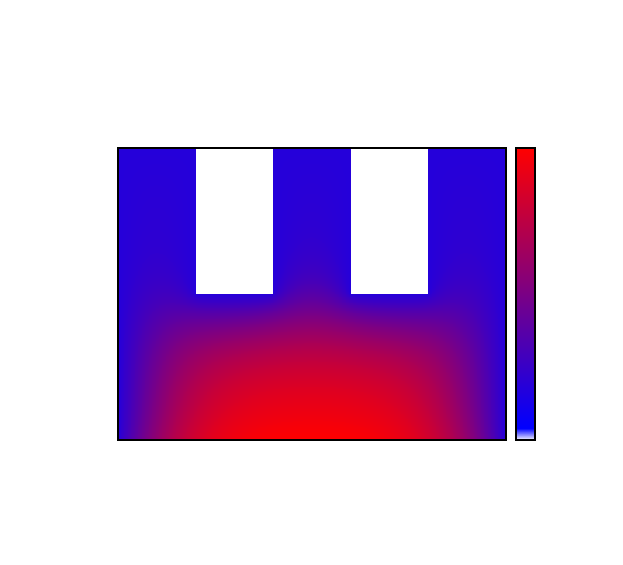
\includegraphics{./figures/heatmap_a_1}}%
    \gplfronttext
  \end{picture}%
\endgroup
}
\vspace{-40pt}
\caption{Temperaturverteilung für $a=0,01$}
\label{fig:a_1}
\vspace{-20pt}
\scalebox{0.9}{% GNUPLOT: LaTeX picture with Postscript
\begingroup
  \makeatletter
  \providecommand\color[2][]{%
    \GenericError{(gnuplot) \space\space\space\@spaces}{%
      Package color not loaded in conjunction with
      terminal option `colourtext'%
    }{See the gnuplot documentation for explanation.%
    }{Either use 'blacktext' in gnuplot or load the package
      color.sty in LaTeX.}%
    \renewcommand\color[2][]{}%
  }%
  \providecommand\includegraphics[2][]{%
    \GenericError{(gnuplot) \space\space\space\@spaces}{%
      Package graphicx or graphics not loaded%
    }{See the gnuplot documentation for explanation.%
    }{The gnuplot epslatex terminal needs graphicx.sty or graphics.sty.}%
    \renewcommand\includegraphics[2][]{}%
  }%
  \providecommand\rotatebox[2]{#2}%
  \@ifundefined{ifGPcolor}{%
    \newif\ifGPcolor
    \GPcolortrue
  }{}%
  \@ifundefined{ifGPblacktext}{%
    \newif\ifGPblacktext
    \GPblacktextfalse
  }{}%
  % define a \g@addto@macro without @ in the name:
  \let\gplgaddtomacro\g@addto@macro
  % define empty templates for all commands taking text:
  \gdef\gplbacktext{}%
  \gdef\gplfronttext{}%
  \makeatother
  \ifGPblacktext
    % no textcolor at all
    \def\colorrgb#1{}%
    \def\colorgray#1{}%
  \else
    % gray or color?
    \ifGPcolor
      \def\colorrgb#1{\color[rgb]{#1}}%
      \def\colorgray#1{\color[gray]{#1}}%
      \expandafter\def\csname LTw\endcsname{\color{white}}%
      \expandafter\def\csname LTb\endcsname{\color{black}}%
      \expandafter\def\csname LTa\endcsname{\color{black}}%
      \expandafter\def\csname LT0\endcsname{\color[rgb]{1,0,0}}%
      \expandafter\def\csname LT1\endcsname{\color[rgb]{0,1,0}}%
      \expandafter\def\csname LT2\endcsname{\color[rgb]{0,0,1}}%
      \expandafter\def\csname LT3\endcsname{\color[rgb]{1,0,1}}%
      \expandafter\def\csname LT4\endcsname{\color[rgb]{0,1,1}}%
      \expandafter\def\csname LT5\endcsname{\color[rgb]{1,1,0}}%
      \expandafter\def\csname LT6\endcsname{\color[rgb]{0,0,0}}%
      \expandafter\def\csname LT7\endcsname{\color[rgb]{1,0.3,0}}%
      \expandafter\def\csname LT8\endcsname{\color[rgb]{0.5,0.5,0.5}}%
    \else
      % gray
      \def\colorrgb#1{\color{black}}%
      \def\colorgray#1{\color[gray]{#1}}%
      \expandafter\def\csname LTw\endcsname{\color{white}}%
      \expandafter\def\csname LTb\endcsname{\color{black}}%
      \expandafter\def\csname LTa\endcsname{\color{black}}%
      \expandafter\def\csname LT0\endcsname{\color{black}}%
      \expandafter\def\csname LT1\endcsname{\color{black}}%
      \expandafter\def\csname LT2\endcsname{\color{black}}%
      \expandafter\def\csname LT3\endcsname{\color{black}}%
      \expandafter\def\csname LT4\endcsname{\color{black}}%
      \expandafter\def\csname LT5\endcsname{\color{black}}%
      \expandafter\def\csname LT6\endcsname{\color{black}}%
      \expandafter\def\csname LT7\endcsname{\color{black}}%
      \expandafter\def\csname LT8\endcsname{\color{black}}%
    \fi
  \fi
  \setlength{\unitlength}{0.0500bp}%
  \begin{picture}(5668.00,5102.00)%
    \gplgaddtomacro\gplbacktext{%
      \csname LTb\endcsname%
      \put(2834,4394){\makebox(0,0){\strut{}Heat Map f{\"u}r Gitterabstand $a=0,1$}}%
    }%
    \gplgaddtomacro\gplfronttext{%
      \csname LTb\endcsname%
      \put(972,752){\makebox(0,0){\strut{}$0$}}%
      \put(1717,752){\makebox(0,0){\strut{}$1$}}%
      \put(2462,752){\makebox(0,0){\strut{}$2$}}%
      \put(3206,752){\makebox(0,0){\strut{}$3$}}%
      \put(3951,752){\makebox(0,0){\strut{}$4$}}%
      \put(4696,752){\makebox(0,0){\strut{}$5$}}%
      \put(801,1038){\makebox(0,0)[r]{\strut{}$0$}}%
      \put(801,1740){\makebox(0,0)[r]{\strut{}$1$}}%
      \put(801,2441){\makebox(0,0)[r]{\strut{}$2$}}%
      \put(801,3142){\makebox(0,0)[r]{\strut{}$3$}}%
      \put(801,3844){\makebox(0,0)[r]{\strut{}$4$}}%
      \put(5107,1630){\makebox(0,0)[l]{\strut{}$0.22$}}%
      \put(5107,3704){\makebox(0,0)[l]{\strut{}$0.29$}}%
      \put(5701,2441){\rotatebox{-270}{\makebox(0,0){\strut{}Temperaturverteilung}}}%
    }%
    \gplbacktext
    \put(0,0){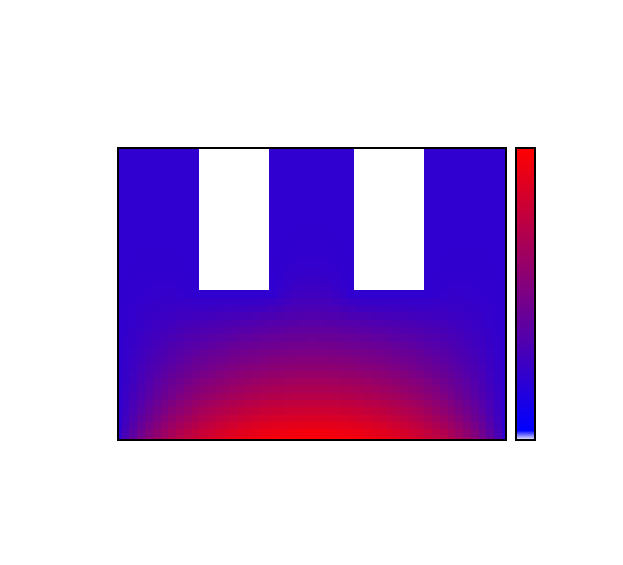
\includegraphics{./figures/heatmap_a_10}}%
    \gplfronttext
  \end{picture}%
\endgroup
}
\vspace{-40pt}
\caption{Temperaturverteilung für $a=0,1$}
\label{fig:a_10}
\end{minipage}
\begin{minipage}[c]{0.5\textwidth}
\centering
\vspace{-60pt}
\scalebox{0.9}{% GNUPLOT: LaTeX picture with Postscript
\begingroup
  \makeatletter
  \providecommand\color[2][]{%
    \GenericError{(gnuplot) \space\space\space\@spaces}{%
      Package color not loaded in conjunction with
      terminal option `colourtext'%
    }{See the gnuplot documentation for explanation.%
    }{Either use 'blacktext' in gnuplot or load the package
      color.sty in LaTeX.}%
    \renewcommand\color[2][]{}%
  }%
  \providecommand\includegraphics[2][]{%
    \GenericError{(gnuplot) \space\space\space\@spaces}{%
      Package graphicx or graphics not loaded%
    }{See the gnuplot documentation for explanation.%
    }{The gnuplot epslatex terminal needs graphicx.sty or graphics.sty.}%
    \renewcommand\includegraphics[2][]{}%
  }%
  \providecommand\rotatebox[2]{#2}%
  \@ifundefined{ifGPcolor}{%
    \newif\ifGPcolor
    \GPcolortrue
  }{}%
  \@ifundefined{ifGPblacktext}{%
    \newif\ifGPblacktext
    \GPblacktextfalse
  }{}%
  % define a \g@addto@macro without @ in the name:
  \let\gplgaddtomacro\g@addto@macro
  % define empty templates for all commands taking text:
  \gdef\gplbacktext{}%
  \gdef\gplfronttext{}%
  \makeatother
  \ifGPblacktext
    % no textcolor at all
    \def\colorrgb#1{}%
    \def\colorgray#1{}%
  \else
    % gray or color?
    \ifGPcolor
      \def\colorrgb#1{\color[rgb]{#1}}%
      \def\colorgray#1{\color[gray]{#1}}%
      \expandafter\def\csname LTw\endcsname{\color{white}}%
      \expandafter\def\csname LTb\endcsname{\color{black}}%
      \expandafter\def\csname LTa\endcsname{\color{black}}%
      \expandafter\def\csname LT0\endcsname{\color[rgb]{1,0,0}}%
      \expandafter\def\csname LT1\endcsname{\color[rgb]{0,1,0}}%
      \expandafter\def\csname LT2\endcsname{\color[rgb]{0,0,1}}%
      \expandafter\def\csname LT3\endcsname{\color[rgb]{1,0,1}}%
      \expandafter\def\csname LT4\endcsname{\color[rgb]{0,1,1}}%
      \expandafter\def\csname LT5\endcsname{\color[rgb]{1,1,0}}%
      \expandafter\def\csname LT6\endcsname{\color[rgb]{0,0,0}}%
      \expandafter\def\csname LT7\endcsname{\color[rgb]{1,0.3,0}}%
      \expandafter\def\csname LT8\endcsname{\color[rgb]{0.5,0.5,0.5}}%
    \else
      % gray
      \def\colorrgb#1{\color{black}}%
      \def\colorgray#1{\color[gray]{#1}}%
      \expandafter\def\csname LTw\endcsname{\color{white}}%
      \expandafter\def\csname LTb\endcsname{\color{black}}%
      \expandafter\def\csname LTa\endcsname{\color{black}}%
      \expandafter\def\csname LT0\endcsname{\color{black}}%
      \expandafter\def\csname LT1\endcsname{\color{black}}%
      \expandafter\def\csname LT2\endcsname{\color{black}}%
      \expandafter\def\csname LT3\endcsname{\color{black}}%
      \expandafter\def\csname LT4\endcsname{\color{black}}%
      \expandafter\def\csname LT5\endcsname{\color{black}}%
      \expandafter\def\csname LT6\endcsname{\color{black}}%
      \expandafter\def\csname LT7\endcsname{\color{black}}%
      \expandafter\def\csname LT8\endcsname{\color{black}}%
    \fi
  \fi
  \setlength{\unitlength}{0.0500bp}%
  \begin{picture}(5668.00,5102.00)%
    \gplgaddtomacro\gplbacktext{%
      \csname LTb\endcsname%
      \put(2834,4394){\makebox(0,0){\strut{}Heat Map f{\"u}r Gitterabstand $a=0,2$}}%
    }%
    \gplgaddtomacro\gplfronttext{%
      \csname LTb\endcsname%
      \put(972,752){\makebox(0,0){\strut{}$0$}}%
      \put(1717,752){\makebox(0,0){\strut{}$1$}}%
      \put(2462,752){\makebox(0,0){\strut{}$2$}}%
      \put(3206,752){\makebox(0,0){\strut{}$3$}}%
      \put(3951,752){\makebox(0,0){\strut{}$4$}}%
      \put(4696,752){\makebox(0,0){\strut{}$5$}}%
      \put(801,1038){\makebox(0,0)[r]{\strut{}$0$}}%
      \put(801,1740){\makebox(0,0)[r]{\strut{}$1$}}%
      \put(801,2441){\makebox(0,0)[r]{\strut{}$2$}}%
      \put(801,3142){\makebox(0,0)[r]{\strut{}$3$}}%
      \put(801,3844){\makebox(0,0)[r]{\strut{}$4$}}%
      \put(5107,1038){\makebox(0,0)[l]{\strut{}$0$}}%
      \put(5107,1369){\makebox(0,0)[l]{\strut{}$0.22$}}%
      \put(5107,3840){\makebox(0,0)[l]{\strut{}$0.37$}}%
      \put(5701,2441){\rotatebox{-270}{\makebox(0,0){\strut{}Temperaturverteilung}}}%
    }%
    \gplbacktext
    \put(0,0){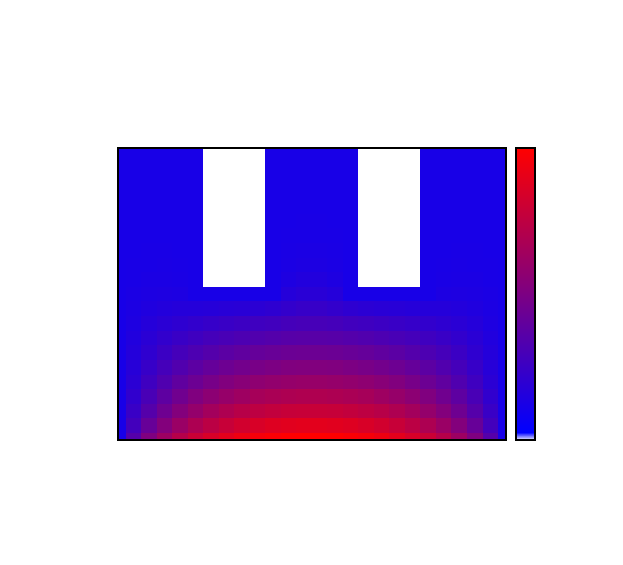
\includegraphics{./figures/heatmap_a_20}}%
    \gplfronttext
  \end{picture}%
\endgroup
}
\vspace{-40pt}
\caption{Temperaturverteilung für $a=0,2$}
\label{fig:a_20}
\vspace{-20pt}
\scalebox{0.9}{% GNUPLOT: LaTeX picture with Postscript
\begingroup
  \makeatletter
  \providecommand\color[2][]{%
    \GenericError{(gnuplot) \space\space\space\@spaces}{%
      Package color not loaded in conjunction with
      terminal option `colourtext'%
    }{See the gnuplot documentation for explanation.%
    }{Either use 'blacktext' in gnuplot or load the package
      color.sty in LaTeX.}%
    \renewcommand\color[2][]{}%
  }%
  \providecommand\includegraphics[2][]{%
    \GenericError{(gnuplot) \space\space\space\@spaces}{%
      Package graphicx or graphics not loaded%
    }{See the gnuplot documentation for explanation.%
    }{The gnuplot epslatex terminal needs graphicx.sty or graphics.sty.}%
    \renewcommand\includegraphics[2][]{}%
  }%
  \providecommand\rotatebox[2]{#2}%
  \@ifundefined{ifGPcolor}{%
    \newif\ifGPcolor
    \GPcolortrue
  }{}%
  \@ifundefined{ifGPblacktext}{%
    \newif\ifGPblacktext
    \GPblacktextfalse
  }{}%
  % define a \g@addto@macro without @ in the name:
  \let\gplgaddtomacro\g@addto@macro
  % define empty templates for all commands taking text:
  \gdef\gplbacktext{}%
  \gdef\gplfronttext{}%
  \makeatother
  \ifGPblacktext
    % no textcolor at all
    \def\colorrgb#1{}%
    \def\colorgray#1{}%
  \else
    % gray or color?
    \ifGPcolor
      \def\colorrgb#1{\color[rgb]{#1}}%
      \def\colorgray#1{\color[gray]{#1}}%
      \expandafter\def\csname LTw\endcsname{\color{white}}%
      \expandafter\def\csname LTb\endcsname{\color{black}}%
      \expandafter\def\csname LTa\endcsname{\color{black}}%
      \expandafter\def\csname LT0\endcsname{\color[rgb]{1,0,0}}%
      \expandafter\def\csname LT1\endcsname{\color[rgb]{0,1,0}}%
      \expandafter\def\csname LT2\endcsname{\color[rgb]{0,0,1}}%
      \expandafter\def\csname LT3\endcsname{\color[rgb]{1,0,1}}%
      \expandafter\def\csname LT4\endcsname{\color[rgb]{0,1,1}}%
      \expandafter\def\csname LT5\endcsname{\color[rgb]{1,1,0}}%
      \expandafter\def\csname LT6\endcsname{\color[rgb]{0,0,0}}%
      \expandafter\def\csname LT7\endcsname{\color[rgb]{1,0.3,0}}%
      \expandafter\def\csname LT8\endcsname{\color[rgb]{0.5,0.5,0.5}}%
    \else
      % gray
      \def\colorrgb#1{\color{black}}%
      \def\colorgray#1{\color[gray]{#1}}%
      \expandafter\def\csname LTw\endcsname{\color{white}}%
      \expandafter\def\csname LTb\endcsname{\color{black}}%
      \expandafter\def\csname LTa\endcsname{\color{black}}%
      \expandafter\def\csname LT0\endcsname{\color{black}}%
      \expandafter\def\csname LT1\endcsname{\color{black}}%
      \expandafter\def\csname LT2\endcsname{\color{black}}%
      \expandafter\def\csname LT3\endcsname{\color{black}}%
      \expandafter\def\csname LT4\endcsname{\color{black}}%
      \expandafter\def\csname LT5\endcsname{\color{black}}%
      \expandafter\def\csname LT6\endcsname{\color{black}}%
      \expandafter\def\csname LT7\endcsname{\color{black}}%
      \expandafter\def\csname LT8\endcsname{\color{black}}%
    \fi
  \fi
  \setlength{\unitlength}{0.0500bp}%
  \begin{picture}(5668.00,5102.00)%
    \gplgaddtomacro\gplbacktext{%
      \csname LTb\endcsname%
      \put(2834,4394){\makebox(0,0){\strut{}Heat Map f{\"u}r Gitterabstand $a=0,25$}}%
    }%
    \gplgaddtomacro\gplfronttext{%
      \csname LTb\endcsname%
      \put(972,752){\makebox(0,0){\strut{}$0$}}%
      \put(1717,752){\makebox(0,0){\strut{}$1$}}%
      \put(2462,752){\makebox(0,0){\strut{}$2$}}%
      \put(3206,752){\makebox(0,0){\strut{}$3$}}%
      \put(3951,752){\makebox(0,0){\strut{}$4$}}%
      \put(4696,752){\makebox(0,0){\strut{}$5$}}%
      \put(801,1038){\makebox(0,0)[r]{\strut{}$0$}}%
      \put(801,1740){\makebox(0,0)[r]{\strut{}$1$}}%
      \put(801,2441){\makebox(0,0)[r]{\strut{}$2$}}%
      \put(801,3142){\makebox(0,0)[r]{\strut{}$3$}}%
      \put(801,3844){\makebox(0,0)[r]{\strut{}$4$}}%
      \put(5107,1309){\makebox(0,0)[l]{\strut{}$0.22$}}%
      \put(5107,3757){\makebox(0,0)[l]{\strut{}$0.40$}}%
      \put(5701,2441){\rotatebox{-270}{\makebox(0,0){\strut{}Temperaturverteilung}}}%
    }%
    \gplbacktext
    \put(0,0){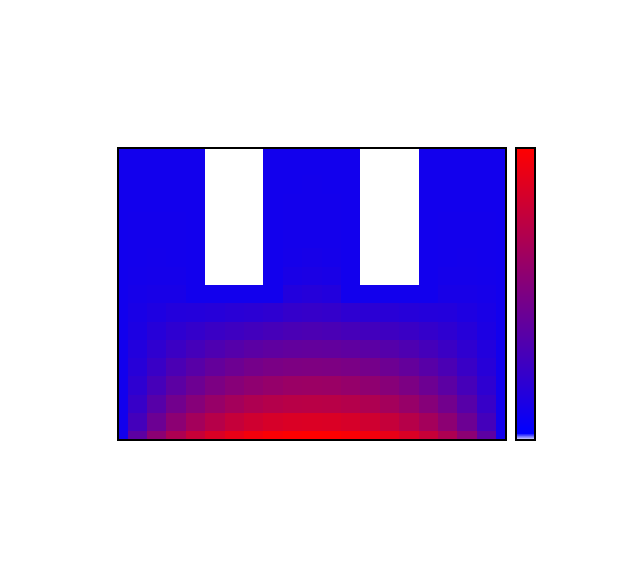
\includegraphics{./figures/heatmap_a_25}}%
    \gplfronttext
  \end{picture}%
\endgroup
}
\vspace{-40pt}
\caption{Temperaturverteilung für $a=0,25$}
\label{fig:a_25}
\end{minipage}
\end{figure}

%\begin{figure}[htbp!]
%\centering
%\vspace{-20pt}
%% GNUPLOT: LaTeX picture with Postscript
\begingroup
  \makeatletter
  \providecommand\color[2][]{%
    \GenericError{(gnuplot) \space\space\space\@spaces}{%
      Package color not loaded in conjunction with
      terminal option `colourtext'%
    }{See the gnuplot documentation for explanation.%
    }{Either use 'blacktext' in gnuplot or load the package
      color.sty in LaTeX.}%
    \renewcommand\color[2][]{}%
  }%
  \providecommand\includegraphics[2][]{%
    \GenericError{(gnuplot) \space\space\space\@spaces}{%
      Package graphicx or graphics not loaded%
    }{See the gnuplot documentation for explanation.%
    }{The gnuplot epslatex terminal needs graphicx.sty or graphics.sty.}%
    \renewcommand\includegraphics[2][]{}%
  }%
  \providecommand\rotatebox[2]{#2}%
  \@ifundefined{ifGPcolor}{%
    \newif\ifGPcolor
    \GPcolortrue
  }{}%
  \@ifundefined{ifGPblacktext}{%
    \newif\ifGPblacktext
    \GPblacktextfalse
  }{}%
  % define a \g@addto@macro without @ in the name:
  \let\gplgaddtomacro\g@addto@macro
  % define empty templates for all commands taking text:
  \gdef\gplbacktext{}%
  \gdef\gplfronttext{}%
  \makeatother
  \ifGPblacktext
    % no textcolor at all
    \def\colorrgb#1{}%
    \def\colorgray#1{}%
  \else
    % gray or color?
    \ifGPcolor
      \def\colorrgb#1{\color[rgb]{#1}}%
      \def\colorgray#1{\color[gray]{#1}}%
      \expandafter\def\csname LTw\endcsname{\color{white}}%
      \expandafter\def\csname LTb\endcsname{\color{black}}%
      \expandafter\def\csname LTa\endcsname{\color{black}}%
      \expandafter\def\csname LT0\endcsname{\color[rgb]{1,0,0}}%
      \expandafter\def\csname LT1\endcsname{\color[rgb]{0,1,0}}%
      \expandafter\def\csname LT2\endcsname{\color[rgb]{0,0,1}}%
      \expandafter\def\csname LT3\endcsname{\color[rgb]{1,0,1}}%
      \expandafter\def\csname LT4\endcsname{\color[rgb]{0,1,1}}%
      \expandafter\def\csname LT5\endcsname{\color[rgb]{1,1,0}}%
      \expandafter\def\csname LT6\endcsname{\color[rgb]{0,0,0}}%
      \expandafter\def\csname LT7\endcsname{\color[rgb]{1,0.3,0}}%
      \expandafter\def\csname LT8\endcsname{\color[rgb]{0.5,0.5,0.5}}%
    \else
      % gray
      \def\colorrgb#1{\color{black}}%
      \def\colorgray#1{\color[gray]{#1}}%
      \expandafter\def\csname LTw\endcsname{\color{white}}%
      \expandafter\def\csname LTb\endcsname{\color{black}}%
      \expandafter\def\csname LTa\endcsname{\color{black}}%
      \expandafter\def\csname LT0\endcsname{\color{black}}%
      \expandafter\def\csname LT1\endcsname{\color{black}}%
      \expandafter\def\csname LT2\endcsname{\color{black}}%
      \expandafter\def\csname LT3\endcsname{\color{black}}%
      \expandafter\def\csname LT4\endcsname{\color{black}}%
      \expandafter\def\csname LT5\endcsname{\color{black}}%
      \expandafter\def\csname LT6\endcsname{\color{black}}%
      \expandafter\def\csname LT7\endcsname{\color{black}}%
      \expandafter\def\csname LT8\endcsname{\color{black}}%
    \fi
  \fi
  \setlength{\unitlength}{0.0500bp}%
  \begin{picture}(5668.00,5102.00)%
    \gplgaddtomacro\gplbacktext{%
      \csname LTb\endcsname%
      %\put(2834,4394){\makebox(0,0){\strut{}Heat Map f{\"u}r Gitterabstand $a=0,01$}}%
    }%
    \gplgaddtomacro\gplfronttext{%
      \csname LTb\endcsname%
      \put(972,752){\makebox(0,0){\strut{}$0$}}%
      \put(1717,752){\makebox(0,0){\strut{}$1$}}%
      \put(2462,752){\makebox(0,0){\strut{}$2$}}%
      \put(3206,752){\makebox(0,0){\strut{}$3$}}%
      \put(3951,752){\makebox(0,0){\strut{}$4$}}%
      \put(4696,752){\makebox(0,0){\strut{}$5$}}%
      \put(801,1038){\makebox(0,0)[r]{\strut{}$0$}}%
      \put(801,1740){\makebox(0,0)[r]{\strut{}$1$}}%
      \put(801,2441){\makebox(0,0)[r]{\strut{}$2$}}%
      \put(801,3142){\makebox(0,0)[r]{\strut{}$3$}}%
      \put(801,3844){\makebox(0,0)[r]{\strut{}$4$}}%
      \put(5107,1545){\makebox(0,0)[l]{\strut{}$0.22$}}%
      \put(5107,3576){\makebox(0,0)[l]{\strut{}$0.24$}}%
      %\put(5701,2441){\rotatebox{-270}{\makebox(0,0){\strut{}Temperaturverteilung}}}%
    }%
    \gplbacktext
    \put(0,0){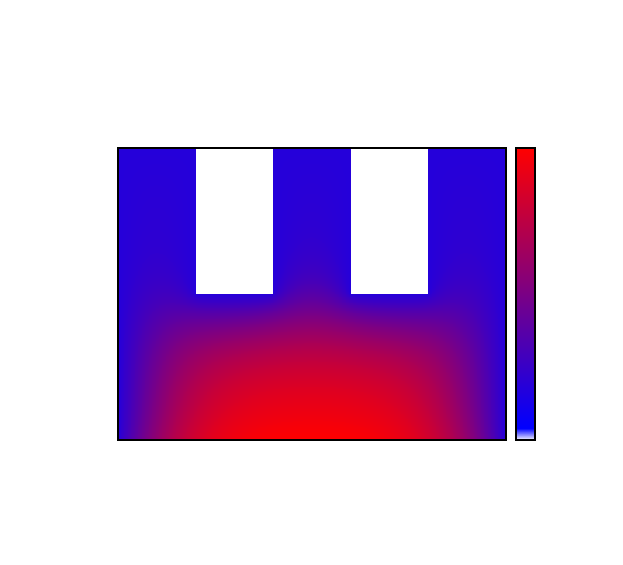
\includegraphics{./figures/heatmap_a_1}}%
    \gplfronttext
  \end{picture}%
\endgroup

%\vspace{-40pt}
%\caption{Temperaturverteilung für $a=0,01$}
%\end{figure}
%\begin{figure}[htbp!]
%\centering
%\vspace{-20pt}
%% GNUPLOT: LaTeX picture with Postscript
\begingroup
  \makeatletter
  \providecommand\color[2][]{%
    \GenericError{(gnuplot) \space\space\space\@spaces}{%
      Package color not loaded in conjunction with
      terminal option `colourtext'%
    }{See the gnuplot documentation for explanation.%
    }{Either use 'blacktext' in gnuplot or load the package
      color.sty in LaTeX.}%
    \renewcommand\color[2][]{}%
  }%
  \providecommand\includegraphics[2][]{%
    \GenericError{(gnuplot) \space\space\space\@spaces}{%
      Package graphicx or graphics not loaded%
    }{See the gnuplot documentation for explanation.%
    }{The gnuplot epslatex terminal needs graphicx.sty or graphics.sty.}%
    \renewcommand\includegraphics[2][]{}%
  }%
  \providecommand\rotatebox[2]{#2}%
  \@ifundefined{ifGPcolor}{%
    \newif\ifGPcolor
    \GPcolortrue
  }{}%
  \@ifundefined{ifGPblacktext}{%
    \newif\ifGPblacktext
    \GPblacktextfalse
  }{}%
  % define a \g@addto@macro without @ in the name:
  \let\gplgaddtomacro\g@addto@macro
  % define empty templates for all commands taking text:
  \gdef\gplbacktext{}%
  \gdef\gplfronttext{}%
  \makeatother
  \ifGPblacktext
    % no textcolor at all
    \def\colorrgb#1{}%
    \def\colorgray#1{}%
  \else
    % gray or color?
    \ifGPcolor
      \def\colorrgb#1{\color[rgb]{#1}}%
      \def\colorgray#1{\color[gray]{#1}}%
      \expandafter\def\csname LTw\endcsname{\color{white}}%
      \expandafter\def\csname LTb\endcsname{\color{black}}%
      \expandafter\def\csname LTa\endcsname{\color{black}}%
      \expandafter\def\csname LT0\endcsname{\color[rgb]{1,0,0}}%
      \expandafter\def\csname LT1\endcsname{\color[rgb]{0,1,0}}%
      \expandafter\def\csname LT2\endcsname{\color[rgb]{0,0,1}}%
      \expandafter\def\csname LT3\endcsname{\color[rgb]{1,0,1}}%
      \expandafter\def\csname LT4\endcsname{\color[rgb]{0,1,1}}%
      \expandafter\def\csname LT5\endcsname{\color[rgb]{1,1,0}}%
      \expandafter\def\csname LT6\endcsname{\color[rgb]{0,0,0}}%
      \expandafter\def\csname LT7\endcsname{\color[rgb]{1,0.3,0}}%
      \expandafter\def\csname LT8\endcsname{\color[rgb]{0.5,0.5,0.5}}%
    \else
      % gray
      \def\colorrgb#1{\color{black}}%
      \def\colorgray#1{\color[gray]{#1}}%
      \expandafter\def\csname LTw\endcsname{\color{white}}%
      \expandafter\def\csname LTb\endcsname{\color{black}}%
      \expandafter\def\csname LTa\endcsname{\color{black}}%
      \expandafter\def\csname LT0\endcsname{\color{black}}%
      \expandafter\def\csname LT1\endcsname{\color{black}}%
      \expandafter\def\csname LT2\endcsname{\color{black}}%
      \expandafter\def\csname LT3\endcsname{\color{black}}%
      \expandafter\def\csname LT4\endcsname{\color{black}}%
      \expandafter\def\csname LT5\endcsname{\color{black}}%
      \expandafter\def\csname LT6\endcsname{\color{black}}%
      \expandafter\def\csname LT7\endcsname{\color{black}}%
      \expandafter\def\csname LT8\endcsname{\color{black}}%
    \fi
  \fi
  \setlength{\unitlength}{0.0500bp}%
  \begin{picture}(5668.00,5102.00)%
    \gplgaddtomacro\gplbacktext{%
      \csname LTb\endcsname%
      \put(2834,4394){\makebox(0,0){\strut{}Heat Map f{\"u}r Gitterabstand $a=0,1$}}%
    }%
    \gplgaddtomacro\gplfronttext{%
      \csname LTb\endcsname%
      \put(972,752){\makebox(0,0){\strut{}$0$}}%
      \put(1717,752){\makebox(0,0){\strut{}$1$}}%
      \put(2462,752){\makebox(0,0){\strut{}$2$}}%
      \put(3206,752){\makebox(0,0){\strut{}$3$}}%
      \put(3951,752){\makebox(0,0){\strut{}$4$}}%
      \put(4696,752){\makebox(0,0){\strut{}$5$}}%
      \put(801,1038){\makebox(0,0)[r]{\strut{}$0$}}%
      \put(801,1740){\makebox(0,0)[r]{\strut{}$1$}}%
      \put(801,2441){\makebox(0,0)[r]{\strut{}$2$}}%
      \put(801,3142){\makebox(0,0)[r]{\strut{}$3$}}%
      \put(801,3844){\makebox(0,0)[r]{\strut{}$4$}}%
      \put(5107,1630){\makebox(0,0)[l]{\strut{}$0.22$}}%
      \put(5107,3704){\makebox(0,0)[l]{\strut{}$0.29$}}%
      \put(5701,2441){\rotatebox{-270}{\makebox(0,0){\strut{}Temperaturverteilung}}}%
    }%
    \gplbacktext
    \put(0,0){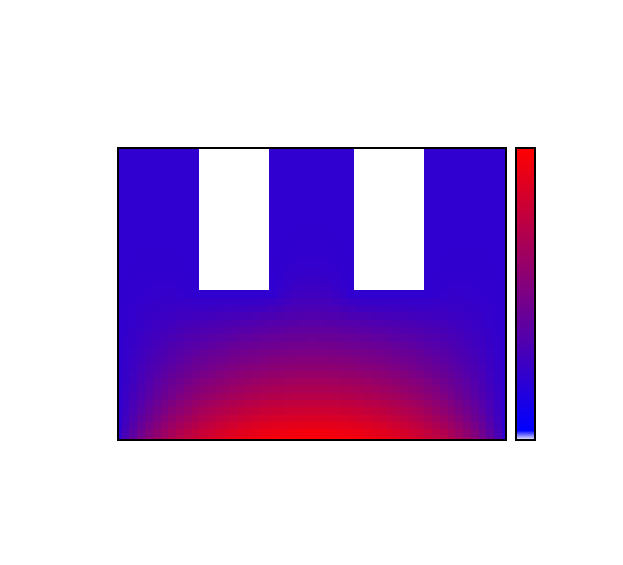
\includegraphics{./figures/heatmap_a_10}}%
    \gplfronttext
  \end{picture}%
\endgroup

%\vspace{-40pt}
%\caption{Temperaturverteilung für $a=0,1$}
%\end{figure}
%\begin{figure}[htbp!]
%\centering
%\vspace{-20pt}
%% GNUPLOT: LaTeX picture with Postscript
\begingroup
  \makeatletter
  \providecommand\color[2][]{%
    \GenericError{(gnuplot) \space\space\space\@spaces}{%
      Package color not loaded in conjunction with
      terminal option `colourtext'%
    }{See the gnuplot documentation for explanation.%
    }{Either use 'blacktext' in gnuplot or load the package
      color.sty in LaTeX.}%
    \renewcommand\color[2][]{}%
  }%
  \providecommand\includegraphics[2][]{%
    \GenericError{(gnuplot) \space\space\space\@spaces}{%
      Package graphicx or graphics not loaded%
    }{See the gnuplot documentation for explanation.%
    }{The gnuplot epslatex terminal needs graphicx.sty or graphics.sty.}%
    \renewcommand\includegraphics[2][]{}%
  }%
  \providecommand\rotatebox[2]{#2}%
  \@ifundefined{ifGPcolor}{%
    \newif\ifGPcolor
    \GPcolortrue
  }{}%
  \@ifundefined{ifGPblacktext}{%
    \newif\ifGPblacktext
    \GPblacktextfalse
  }{}%
  % define a \g@addto@macro without @ in the name:
  \let\gplgaddtomacro\g@addto@macro
  % define empty templates for all commands taking text:
  \gdef\gplbacktext{}%
  \gdef\gplfronttext{}%
  \makeatother
  \ifGPblacktext
    % no textcolor at all
    \def\colorrgb#1{}%
    \def\colorgray#1{}%
  \else
    % gray or color?
    \ifGPcolor
      \def\colorrgb#1{\color[rgb]{#1}}%
      \def\colorgray#1{\color[gray]{#1}}%
      \expandafter\def\csname LTw\endcsname{\color{white}}%
      \expandafter\def\csname LTb\endcsname{\color{black}}%
      \expandafter\def\csname LTa\endcsname{\color{black}}%
      \expandafter\def\csname LT0\endcsname{\color[rgb]{1,0,0}}%
      \expandafter\def\csname LT1\endcsname{\color[rgb]{0,1,0}}%
      \expandafter\def\csname LT2\endcsname{\color[rgb]{0,0,1}}%
      \expandafter\def\csname LT3\endcsname{\color[rgb]{1,0,1}}%
      \expandafter\def\csname LT4\endcsname{\color[rgb]{0,1,1}}%
      \expandafter\def\csname LT5\endcsname{\color[rgb]{1,1,0}}%
      \expandafter\def\csname LT6\endcsname{\color[rgb]{0,0,0}}%
      \expandafter\def\csname LT7\endcsname{\color[rgb]{1,0.3,0}}%
      \expandafter\def\csname LT8\endcsname{\color[rgb]{0.5,0.5,0.5}}%
    \else
      % gray
      \def\colorrgb#1{\color{black}}%
      \def\colorgray#1{\color[gray]{#1}}%
      \expandafter\def\csname LTw\endcsname{\color{white}}%
      \expandafter\def\csname LTb\endcsname{\color{black}}%
      \expandafter\def\csname LTa\endcsname{\color{black}}%
      \expandafter\def\csname LT0\endcsname{\color{black}}%
      \expandafter\def\csname LT1\endcsname{\color{black}}%
      \expandafter\def\csname LT2\endcsname{\color{black}}%
      \expandafter\def\csname LT3\endcsname{\color{black}}%
      \expandafter\def\csname LT4\endcsname{\color{black}}%
      \expandafter\def\csname LT5\endcsname{\color{black}}%
      \expandafter\def\csname LT6\endcsname{\color{black}}%
      \expandafter\def\csname LT7\endcsname{\color{black}}%
      \expandafter\def\csname LT8\endcsname{\color{black}}%
    \fi
  \fi
  \setlength{\unitlength}{0.0500bp}%
  \begin{picture}(5668.00,5102.00)%
    \gplgaddtomacro\gplbacktext{%
      \csname LTb\endcsname%
      \put(2834,4394){\makebox(0,0){\strut{}Heat Map f{\"u}r Gitterabstand $a=0,2$}}%
    }%
    \gplgaddtomacro\gplfronttext{%
      \csname LTb\endcsname%
      \put(972,752){\makebox(0,0){\strut{}$0$}}%
      \put(1717,752){\makebox(0,0){\strut{}$1$}}%
      \put(2462,752){\makebox(0,0){\strut{}$2$}}%
      \put(3206,752){\makebox(0,0){\strut{}$3$}}%
      \put(3951,752){\makebox(0,0){\strut{}$4$}}%
      \put(4696,752){\makebox(0,0){\strut{}$5$}}%
      \put(801,1038){\makebox(0,0)[r]{\strut{}$0$}}%
      \put(801,1740){\makebox(0,0)[r]{\strut{}$1$}}%
      \put(801,2441){\makebox(0,0)[r]{\strut{}$2$}}%
      \put(801,3142){\makebox(0,0)[r]{\strut{}$3$}}%
      \put(801,3844){\makebox(0,0)[r]{\strut{}$4$}}%
      \put(5107,1038){\makebox(0,0)[l]{\strut{}$0$}}%
      \put(5107,1369){\makebox(0,0)[l]{\strut{}$0.22$}}%
      \put(5107,3840){\makebox(0,0)[l]{\strut{}$0.37$}}%
      \put(5701,2441){\rotatebox{-270}{\makebox(0,0){\strut{}Temperaturverteilung}}}%
    }%
    \gplbacktext
    \put(0,0){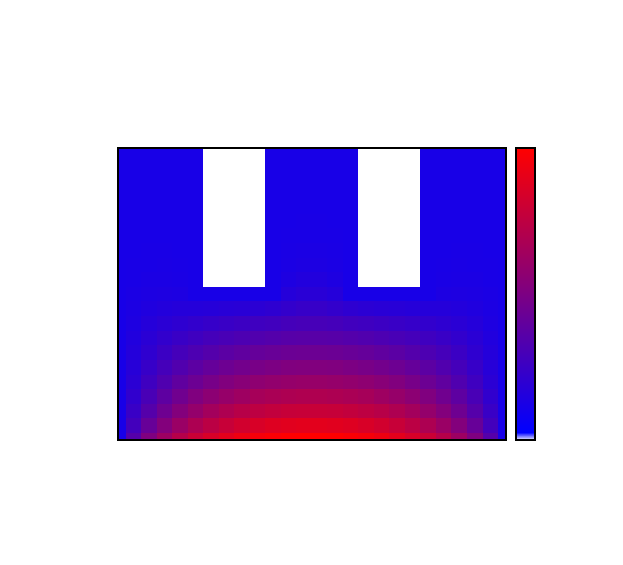
\includegraphics{./figures/heatmap_a_20}}%
    \gplfronttext
  \end{picture}%
\endgroup

%\vspace{-40pt}
%\caption{Temperaturverteilung für $a=0,2$}
%\end{figure}
%\begin{figure}[htbp!]
%\centering
%\vspace{-20pt}
%% GNUPLOT: LaTeX picture with Postscript
\begingroup
  \makeatletter
  \providecommand\color[2][]{%
    \GenericError{(gnuplot) \space\space\space\@spaces}{%
      Package color not loaded in conjunction with
      terminal option `colourtext'%
    }{See the gnuplot documentation for explanation.%
    }{Either use 'blacktext' in gnuplot or load the package
      color.sty in LaTeX.}%
    \renewcommand\color[2][]{}%
  }%
  \providecommand\includegraphics[2][]{%
    \GenericError{(gnuplot) \space\space\space\@spaces}{%
      Package graphicx or graphics not loaded%
    }{See the gnuplot documentation for explanation.%
    }{The gnuplot epslatex terminal needs graphicx.sty or graphics.sty.}%
    \renewcommand\includegraphics[2][]{}%
  }%
  \providecommand\rotatebox[2]{#2}%
  \@ifundefined{ifGPcolor}{%
    \newif\ifGPcolor
    \GPcolortrue
  }{}%
  \@ifundefined{ifGPblacktext}{%
    \newif\ifGPblacktext
    \GPblacktextfalse
  }{}%
  % define a \g@addto@macro without @ in the name:
  \let\gplgaddtomacro\g@addto@macro
  % define empty templates for all commands taking text:
  \gdef\gplbacktext{}%
  \gdef\gplfronttext{}%
  \makeatother
  \ifGPblacktext
    % no textcolor at all
    \def\colorrgb#1{}%
    \def\colorgray#1{}%
  \else
    % gray or color?
    \ifGPcolor
      \def\colorrgb#1{\color[rgb]{#1}}%
      \def\colorgray#1{\color[gray]{#1}}%
      \expandafter\def\csname LTw\endcsname{\color{white}}%
      \expandafter\def\csname LTb\endcsname{\color{black}}%
      \expandafter\def\csname LTa\endcsname{\color{black}}%
      \expandafter\def\csname LT0\endcsname{\color[rgb]{1,0,0}}%
      \expandafter\def\csname LT1\endcsname{\color[rgb]{0,1,0}}%
      \expandafter\def\csname LT2\endcsname{\color[rgb]{0,0,1}}%
      \expandafter\def\csname LT3\endcsname{\color[rgb]{1,0,1}}%
      \expandafter\def\csname LT4\endcsname{\color[rgb]{0,1,1}}%
      \expandafter\def\csname LT5\endcsname{\color[rgb]{1,1,0}}%
      \expandafter\def\csname LT6\endcsname{\color[rgb]{0,0,0}}%
      \expandafter\def\csname LT7\endcsname{\color[rgb]{1,0.3,0}}%
      \expandafter\def\csname LT8\endcsname{\color[rgb]{0.5,0.5,0.5}}%
    \else
      % gray
      \def\colorrgb#1{\color{black}}%
      \def\colorgray#1{\color[gray]{#1}}%
      \expandafter\def\csname LTw\endcsname{\color{white}}%
      \expandafter\def\csname LTb\endcsname{\color{black}}%
      \expandafter\def\csname LTa\endcsname{\color{black}}%
      \expandafter\def\csname LT0\endcsname{\color{black}}%
      \expandafter\def\csname LT1\endcsname{\color{black}}%
      \expandafter\def\csname LT2\endcsname{\color{black}}%
      \expandafter\def\csname LT3\endcsname{\color{black}}%
      \expandafter\def\csname LT4\endcsname{\color{black}}%
      \expandafter\def\csname LT5\endcsname{\color{black}}%
      \expandafter\def\csname LT6\endcsname{\color{black}}%
      \expandafter\def\csname LT7\endcsname{\color{black}}%
      \expandafter\def\csname LT8\endcsname{\color{black}}%
    \fi
  \fi
  \setlength{\unitlength}{0.0500bp}%
  \begin{picture}(5668.00,5102.00)%
    \gplgaddtomacro\gplbacktext{%
      \csname LTb\endcsname%
      \put(2834,4394){\makebox(0,0){\strut{}Heat Map f{\"u}r Gitterabstand $a=0,25$}}%
    }%
    \gplgaddtomacro\gplfronttext{%
      \csname LTb\endcsname%
      \put(972,752){\makebox(0,0){\strut{}$0$}}%
      \put(1717,752){\makebox(0,0){\strut{}$1$}}%
      \put(2462,752){\makebox(0,0){\strut{}$2$}}%
      \put(3206,752){\makebox(0,0){\strut{}$3$}}%
      \put(3951,752){\makebox(0,0){\strut{}$4$}}%
      \put(4696,752){\makebox(0,0){\strut{}$5$}}%
      \put(801,1038){\makebox(0,0)[r]{\strut{}$0$}}%
      \put(801,1740){\makebox(0,0)[r]{\strut{}$1$}}%
      \put(801,2441){\makebox(0,0)[r]{\strut{}$2$}}%
      \put(801,3142){\makebox(0,0)[r]{\strut{}$3$}}%
      \put(801,3844){\makebox(0,0)[r]{\strut{}$4$}}%
      \put(5107,1309){\makebox(0,0)[l]{\strut{}$0.22$}}%
      \put(5107,3757){\makebox(0,0)[l]{\strut{}$0.40$}}%
      \put(5701,2441){\rotatebox{-270}{\makebox(0,0){\strut{}Temperaturverteilung}}}%
    }%
    \gplbacktext
    \put(0,0){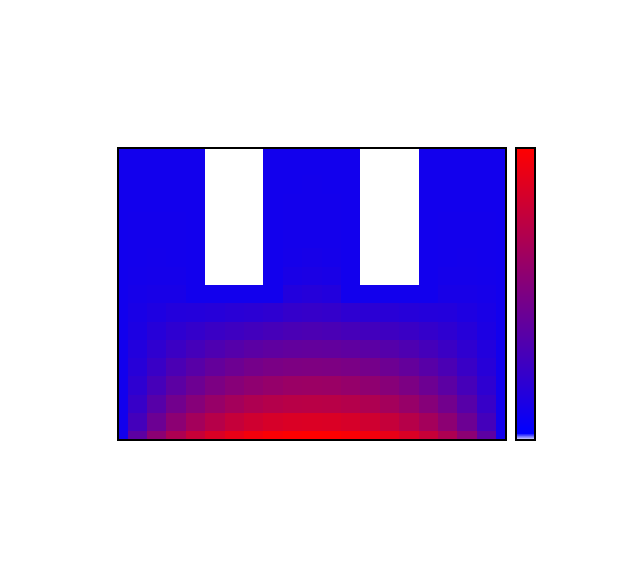
\includegraphics{./figures/heatmap_a_25}}%
    \gplfronttext
  \end{picture}%
\endgroup

%\vspace{-40pt}
%\caption{Temperaturverteilung für $a=0,25$}
%\end{figure}

Auffällig ist, dass mit sinkendem Gitterabstand die maximale Temperatur sinkt. Außerdem sieht man besonders beim Übergang von $a=0,1$  zu $a=0,01$ gut, dass der Bereich mittlerer Temperaturen kleiner wird, da die rot gefärbte Fläche größer und die Ränder schmäler werden.

In Abbildung \ref{fig:a_1} sind die weißen Flächen deutlich breiter als bei den anderen Darstellungen, was in der Diskretisierung begründet ist. Es wird ein Quadrat mit Kantenlänge $a$ um jeden Gitterpunkt gelegt, was dazu führt, dass bei großem Gitterabstand die Quadrate eine größere Kantenlänge haben und von ihrem zugeordneten Punkt ausgehend in das ausgenommene (=weiße) Gebiet "`hineinragen"'. Dieser Effekt tritt eigentlich in allen Abbildungen auf, ist aber aufgrund der nah beieinander liegenden $a$ in Abbildungen \ref{fig:a_10}, \ref{fig:a_20}, \ref{fig:a_25} schwerer zu erkennen.
\end{document}
